\chapter{Introduction}

Programma:
\begin{itemize}
    \item Teoria dell'Informazione
    \item Teoria della Complessità
    \item Algoritmi su Grafi ecc \dots
\end{itemize}





%%%%%%%%%%%%%%%%%%
\chapter{Teoria dell'Informazione}

\section{Entropia}
% LEZIONE 1
Claude Shannon, 1948, \textit{A Mathematical Theory of Communication}.

Un messaggio è una sequenza di lettere (simboli) da un alfabeto. Qual è l'informazione in una frase (messaggio)? Come possiamo misurare la quantità di informazione? Dipende dal contesto.

\subparagraph{Esempio} Il messaggio è ``Piove!''. Qual è la quantità di informazione? Per il signor Muller, che vive a Vienna, dove piove spesso, la quantità di informazione è bassa. Per Fatima, che vive nel deserto, invece, è alta.\bigskip

Si ha quindi che
\begin{itemize}
    \item Bassa probabilità di un evento 
\end{itemize}

...

% LEZIONE 2
\section{Teorema di Bayes}
Sappiamo che nel caso di due \textbf{eventi indipendenti}, la probabilità congiunta è
$$
    p(a_i,b_j) = p(a_i)\cdot p(b_j)
$$
Nel caso, invece, di due \textbf{eventi dipendenti} si ha
$$
    p(a_i,b_j) = p(a_i|b_j)\cdot p(b_j) = p(b_j|a_i)\cdot p(a_i)
$$
e quindi
$$
p(a_i|b_j) = \dfrac{p(b_j|a_i)\cdot p(a_i)}{p(b_j)}
$$
con $p(b_j)$ fattore di normalizzazione.

\textcolor{Red}{TODO: vedere al capitolo 2 del libro il prior, poterior, likelihood, ecc.}



\section{Proprietà dell'Entropia}
Libro, pag.~33. Le proprietà della funzione di entropia sono:
\begin{itemize}
    \item $H(P)\geq 0$ con uguaglianza iff $p_i=1$ per un qualche $i$. In particolare, $H(P)=0$ iff $\exists i ~p_i=1$, ovvero quando c'è un evento certo l'entropia è nulla.
    \item L'entropia è massimizzata se la distribuzione $p$ è uniforme.
\end{itemize}
Analizziamo meglio e dimostriamo la seconda proprietà.

\begin{property}[Entropia massima] 
    $$
        \mathcal{H}(P)\leq \log_2|P|
    $$
    con $|P|$ numero di eventi ($|X|$), e
    $$
        \mathcal{H}\left(\frac{1}{k},\frac{1}{k},\dots,\frac{1}{k}\right) = \log_2 k
    $$
    dove $k$ è il numero di eventi, ovvero $|P|$.
\end{property}

\subparagraph{Dimostrazione} La dimostrazione è basata su proprietà di funzioni complesse, in particolare sulla diseguaglianza di Jensen, la quale è una disuguaglianza che lega il valore di una funzione convessa al valore della medesima funzione calcolata nel valor medio del suo argomento.

Sia $\bm{f(x)=-x\log_2x}$ (cfr.~definizione di entropia). Vogliamo controllare se è concava o convessa, calcoliamo quindi la sua derivata seconda:
$$
    f''(x) = -\frac{1}{x}
$$
Sappiamo che $0\leq x\leq 1$ perché è una probabilità, e quindi abbiamo che $-\nicefrac{1}{x}<0$: la funzione è con\-ca\-va. Prendiamo ora due punti $x_1$ e $x_2$, e un punto $x$ tra i due.
% $0\leq-\nicefrac{1}{x}\leq 1$ perché è una probabilità, e quindi abbiamo che $x<0$: la funzione è concava. Prendiamo ora due punti $x_1$ e $x_2$, e un punto $x$ tra i due.

\textcolor{Red}{TODO: disegno}

Abbiamo che la media pesata di $x_1$ e $x_2$ è
$$
    x = \lambda x_1 + (1-\lambda)x_2 \qquad \text{con} \quad 0\leq\lambda\leq 1
$$
con $\lambda$ il peso. In particolare, se $\lambda=1$ allora $x=x_1$, se $\lambda=0$ allora $x=x_2$, e se $\lambda=\nicefrac{1}{2}$ allora $x$ si troverà esattamente a metà tra $x_1$ e $x_2$. Se prendiamo la combinazione lineare di $f(x_1)$ e $f(x_2)$, otteniamo la seguente di\-su\-gua\-glian\-za:
$$
    \lambda f(x_1) + (1-\lambda)f(x_2) \leq f(\lambda x_1 + (1-\lambda)x_2)
$$
Tale disuguaglianza si può generalizzare alla combinazione lineare di un qualsiasi numero di punti. Se $f''(x)\leq 0$, $\forall x\in[x_1,x_n]$ (ovvero $f''(x)$ è concava) si ha la disuguaglianza di Jensen: 
$$
\textcolor{ForestGreen}{\sum_{i=1}^n\lambda_if(x_i)} \leq \textcolor{Cerulean}{f\left(\sum_{i=1}^n\lambda_ix_i\right)}
$$
con $\lambda_i\geq0$ e $\sum_{i=1}^n\lambda_i=1$. La disuguaglianza cambia verso ($\geq$) quando la funzione è convessa, cioè $f''(x)\geq 0$. Ricordiamo che vogliamo arrivare alla combinazione lineare dove i punti hanno la stessa probabilità. Quindi con
$$
    \lambda_i=\frac{1}{k} \qquad\qquad |P|=|X|=k \qquad\qquad P=\{p_1,\dots,p_k\}
$$
scriviamo la disuguaglianza di Jensen come
\begin{eqnarray*}
    \textcolor{ForestGreen}{\sum_{i=1}^k\underbrace{\frac{1}{k}}_{\lambda_i}\underbrace{(-p_i\log_2p_i)}_{f(x_i)}} & \leq & \underbrace{\textcolor{Cerulean}{-\left(\sum_{i=1}^k\frac{1}{k}p_i\right)\log_2\left(\sum_{i=1}^k\frac{1}{k}p_i\right)}}_{f(\sum\lambda_ix_i)}\\
    -\cancelto{\text{\footnotesize semplifichiamo perché $k>0$}}{\frac{1}{k}}\sum_{i=1}^kp_i\log_2p_i & \leq & -\cancel{\frac{1}{k}}\log_2\frac{1}{k}\\
    \mathcal{H}(P) & \leq & \log_2k=\mathcal{H}\left(\frac{1}{k},\dots,\frac{1}{k}\right)
\end{eqnarray*}
Ovvero l'entropia è massima per la distribuzione uniforme. \hfill$\Box$\bigskip 

\begin{property}[Entropia Congiunta]
    Siano $P,Q$ due distribuzioni, e $x_i,y_j$ coppia di eventi tali che $x_i\in P$ e $y_j\in Q$. L'entropia congiunta di $P,Q$ è:
    $$
        \mathcal{H}(P,Q) = -\sum_{i,j}p(x_i,y_j)\log_2(p(x_i,y_j))
    $$
    Se $x$ e $y$ sono indipendenti (quindi la probabilità congiunta è il prodotto delle due probabilità) l'entropia è additiva:
    $$
        \mathcal{H}(P,Q) = \mathcal{H}(P) + \mathcal{H}(Q)
        % ESERCIZIO ESAME
    $$
\end{property}
La somma è possibile perché usiamo i logaritmi, e una delle loro proprietà è $\log(a\cdot b)=\log(a)+\log(b)$.


\subsection{Scomponibilità dell'Entropia}
Libro, pag.~33. Sia $P$ una distribuzione (vettore) di probabilità, e $X$ delle variabili.
\begin{eqnarray*}
    P &=& \{ p_1,~p_2,~...,~p_n\}\\
    X &=& \{ \underbrace{x_1}_{p_1},\underbrace{x_2,...,x_n}_{1-p_1}\}
\end{eqnarray*}
In questo contesto, la probabilità, ad esempio, del secondo evento $x_2$ è, normalizzata, pari a $\nicefrac{p_2}{1-p_1}$, e quella dell'ultimo elemento $x_n$ è $\nicefrac{p_n}{1-p_1}$.

\subparagraph{Esempio} Abbiamo una moneta regolare. Al primo lancio esce $H$, e come risultati desiderati per il secondo e terzo lancio vogliamo $T$ e $T$. Abbiamo quindi:
\begin{eqnarray*}
    \underbrace{H}_{\substack{p_1=\frac{1}{2}\\\frac{1}{2}}}~\underbrace{T\quad T}_{\substack{1-p_1=\frac{1}{2}\\\frac{1}{4}\quad\frac{1}{4}}}
\end{eqnarray*}

La quantità di informazione ricevuta da $P$ è uguale a quella ricevuta dal processo in due passaggi.
\begin{eqnarray*}
    \mathcal{H}(P)  & = & \sum p_i\log_2\frac{1}{p_i}\\
                    & = & \underbrace{\mathcal{H}(p_1,1-p_1)+(1-p_1)\cdot\mathcal{H}\underbrace{\left(\frac{p_2}{1-p_1},\frac{p_3}{1-p_1},\dots,\frac{p_n}{1-p_1}\right)}_{\substack{\text{$p_i$ normalizzati la cui somma è 1}\\1-p_1=p_2+p_3+\dots+p_n}}}_{\text{si possono dividere in diversi punti, ottenendo, ad esempio, tante entropie}}
\end{eqnarray*}

\textcolor{Red}{TODO: vdere proprietà libro pag 33 sez 2.6?}


\section{Inferenza}
\textcolor{Red}{TODO: capitolo 3, esercizio 3.8 pag 57}

\section{Compressione}
\textcolor{Red}{TODO: capitolo 4, esercizio 4.1 pag 66}


\section{Il Teorema Della Codifica Sorgente}
Studiamo $\mathcal{H}(\{p,1-p\})$, con $0\leq p\leq 1$
\begin{eqnarray*}
    \mathcal{H}(\{p,1-p\})  & = &\\
                            & = & p\log\frac{1}{p} + (1-p)\log\frac{1}{1-p}\\
                            & = & -p\log(p) - (1-p)\log(1-p)\\
                            & = & \mathcal{H}(p)
\end{eqnarray*}

\textcolor{Red}{TODO: finire}


\textcolor{Red}{LEZ 3}

\textcolor{Red}{TODO: soluzione esercizio 4.1}

\textcolor{Red}{TODO: muddy children puzzle}



\section{Codici Simbolo}

\begin{definition}[Alfabeti di input/output]
    \begin{align*}
        \text{Alfabeto di input} \quad &\mathcal{A}=\{a_1,a_2,\dots,a_k\}\\
        \text{Alfabeto di output} \quad &\mathcal{B}=\{b_1,b_2,\dots,b_D\}\\
    \end{align*}
\end{definition}

\begin{definition}[Codice]
    Sia $\mathcal{A}^*$ un messaggio (sequenza di caratteri) sull'alfabeto $\mathcal{A}$. Il \textbf{codice} $c$ è
    $$
        c:\mathcal{A}^*\to\mathcal{B}^*
    $$
    ovvero un messaggio dall'alfabeto $\mathcal{A}$ all'alfabeto $\mathcal{B}$ (iniettiva).
\end{definition}
Con $\mathcal{A}^*=\bigcup_{n\in\mathbb{N}}A^n$, ovvero l'insieme di tutte le possibili stringhe che si possono creare utilizzando l'alfabeto $\mathcal{A}$, compresa la stringa vuota.\medskip 

Si vuole comprimere il messaggio in modo da ottenere il messaggio più corto possibile. Per farlo, utilizziamo una codifica.
\begin{definition}[Codifica]
    Una codifica è una funzione 
    $$
        \varphi:\mathcal{A}\to\mathcal{B}^*
    $$ 
    Inoltre
    $$
        \varphi(\underbrace{x_1,x_2,\dots,x_m}_{\in\mathcal{A}^*}) = \varphi(x_1)\varphi(x_2)\dots\varphi(x_m)
    $$
\end{definition}

\paragraph{Esempio 1} Alfabeti: $\mathcal{A}=\{a,b,c\}$, $\mathcal{B}=\{0,1\}$; codifica: $\varphi(a)=0$, $\varphi(b)=10$, $\varphi(c)=01$. È una buona codifica? No, perché è ambigua. Ad esempio
$$
    \varphi(ab) = 010 = \varphi(ca)
$$
È iniettiva nella codifica ma non sul messaggio. Una codifica di questo tipo viene detta \textbf{not uniquely decodable} (non univocamente decodificabile).

\begin{definition}[Univocamente decodificabile]
    Un codice $\varphi:\mathcal{A}\to\mathcal{B}^*$ è univocamente decodificabile (uniquely decodable) se
    $$
        \forall m_1,m_2\in\mathcal{A}^* \qquad \varphi(m_1)\neq\varphi(m_2)
    $$
\end{definition}
In questo corso non utilizzeremo codici non univocamente decodificabili.

\paragraph{Esempio 2} Alfabeti: $\mathcal{A}=\{a,b,c\}$, $\mathcal{B}=\{0,1\}$; codifica: $\varphi(a)=0$, $\varphi(b)=01$, $\varphi(c)=011$. Ad esempio, il messaggio $aabcbbca$ viene codificato come $\varphi(aabcbbca)=000101101010110$. È univocamente decodificabile (UD)?

Sì, è UD con delay 1. Ad ogni 0, si controlla il carattere successivo: se è un altro 0, la lettera è $a$, altrimenti si prosegue fino al primo 1 per decidere se è $b$ o $c$. Il delay 1 è riferito allo zero che si incontra, che significa l'inizio di un'altra lettera.

\paragraph{Esempio 3} Alfabeti: $\mathcal{A}=\{a,b,c\}$, $\mathcal{B}=\{0,1\}$; codifica: $\varphi(a)=00$, $\varphi(b)=1$, $\varphi(c)=10$. Ad esempio, il messaggio $bcbaca$ viene codificato come $\varphi(bcbaca)=1101001000$. È UD? 

Sì, si controlla se c'è un numero pari o dispari di 0 dopo un 1: se è pari, si tratta di una $b$ seguita da una o più $a$, se è dispari di una $c$, eventualmente seguita da una o più $a$. È UD con unbounded delay.\bigskip 

Abbiamo visto che nel caso di distribuzione uniforme, la quantità di informazione è pari all'entropia. Quanto è complesso computare una codifica/decodifica?

Poiché l'alfabeto di input è binario, per rappresentare una codifica si può utilizzare un albero binario. Quello per l'\textbf{Esempio 2} è il seguente:
\begin{center}
    \begin{tikzpicture}[grow=right]
        \node {$\bullet$}
        child {
            node {$\bullet$}        
            edge from parent 
            node[below] {$1$}
        }
        child {
            node {$a$}        
            child {
                    node {$b$}
                    child {
                        node {$c$}
                        edge from parent
                        node[below] {$1$}
                    }
                    child {
                        node {$\bullet$}
                        edge from parent
                        node[above] {$0$}
                    }
                    edge from parent
                    node[below] {$1$}
                }
                child {
                    node {$\bullet$}
                    edge from parent
                    node[above] {$0$}
                }
            edge from parent         
            node[above] {$0$}
        };
    \end{tikzpicture}
\end{center}
Quello per l'\textbf{Esempio 3} è il seguente: \textcolor{Red}{TODO: fixare in modo che gli archi ad $a$ e $c$ siano inclinati}
\begin{center}
    \begin{tikzpicture}[grow=right]
        \node {$\bullet$}
        child {
            node {$b$}
            child {
                node {$c$}        
                edge from parent 
                node[below] {$0$}
            }        
            edge from parent 
            node[below] {$1$}
        }
        child {
            node {$\bullet$} 
            child {
                node {$a$}
                edge from parent
                node[above] {$0$}
            }
            edge from parent         
            node[above] {$0$}
        };
    \end{tikzpicture}
\end{center}
Quando si finisce in un nodo con un'etichetta ci si deve chiedere se la conclusione è che ci si può fermare. Il grado (fattore) di diramazione è pari alla cardinalità dell'alfabeto di output. Inoltre, se l'albero ha altezza $h$, tutte le codifiche hanno lunghezza $h$.

Ci chiediamo, qual è una codifica sicuramente UD e senza delay?

\begin{definition}[Codice prefisso]
    \begin{eqnarray*}
        &\varphi : \mathcal{A} \to \mathcal{B}^* \text{ è un codice prefisso}&\\
        &\Updownarrow&\\
        &\forall a_i,a_j\in\mathcal{A} \quad \varphi(a_i)\in\mathcal{B}^*\text{ non è un prefisso di }\varphi(a_j)\in\mathcal{B}^*&
    \end{eqnarray*}
\end{definition}
Al posto di codice prefisso (prefix code) utilizzeremo il termine prefisso (prefix). \textcolor{Red}{è corretto?}

\paragraph{Esempio 3 (vedi sopra)} $\varphi$ non è un prefisso, perché la codifica di $b$ è $1$, che è un prefisso della codifica di $c$, ovvero 10.

\begin{lemma}
    $\varphi$ è un codice prefisso \quad $\Rightarrow$ \quad $\varphi$ è UD senza delay
\end{lemma}
Per memorizzare l'albero si utilizza CONSTANT SPACE, che è un sottoinsieme di LINEAR TIME. Ciò equivale a dire che è possibile computarlo con un automa.

\paragraph{Esempio 3 (vedi sopra)} $\varphi(bbb)=111$: il messaggio di input ha lunghezza 3, e viene codificato in un messaggio di lunghezza uguale (3). 

$\varphi(aca)=001000$: il messaggio di input ha lunghezza 3, e viene codificato in un messaggio di lunghezza 6.

Il numero di possibili messaggi di lunghezza 3 in output è $2^3=8$.

\begin{definition}[Lunghezza media di una codifica, EL (Expected Length)]
    Siano $\varphi:\mathcal{A}\to\mathcal{B}^*$ una codifica, e $P$ una distribuzione di probabilità sull'alfabeto di input $\mathcal{A}$
    $$
        EL(\varphi) = \sum_{i=1}^n p(a_i)\cdot|\varphi(a_i)|
    $$
    con $|\varphi(a_i)|=l_i$ lunghezza della codifica di $a_i$.
\end{definition}

\paragraph{Esempio} Supponiamo che nell'\textbf{Esempio 3} le probabilità siano $p(a)=\nicefrac{1}{2}$, $p(b)=\nicefrac{1}{4}$, $p(c)=\nicefrac{1}{4}$. La lunghezza media è
$$
    EL(\varphi) = \frac{1}{2}\cdot 2 + \frac{1}{4}\cdot 1 + \frac{1}{4}\cdot 2 = 1+\frac{3}{4}
$$
Immaginiamo una codifica $\varphi^*$ diversa, per la quale $|\varphi^*(a)|=1$, $|\varphi^*(b)|=2$, $|\varphi^*(c)|=2$. La lunghezza media è
$$
    EL(\varphi^*) = \frac{1}{2}\cdot 1 + \frac{1}{4}\cdot 2 + \frac{1}{4}\cdot 2 = \frac{3}{2}
$$
Abbiamo che $EL(\varphi)>EL(\varphi^*)$, quindi $\varphi^*$ è migliore di $\varphi$.\bigskip

Si vuole trovare la codifica con la minor EL sotto l'assunzione che la sorgente del messaggio non abbia memoria. Dati $\mathcal{A}$, $\mathcal{B}^*$, $P$, si vuole trovare la miglior codifica $\varphi$. Non è sufficiente considerare solo codici prefix-free.

Possiamo raggiungere il minimo di EL considerando i codici prefisso. EL è codificata da $\mathcal{H}(P)$. I codici possono essere asintotticamente ottimali, o ottimali.


\section{Limite imposto dalla Decodificabilità Univoca}

È possibile definire un codice $\varphi:\mathcal{A}\to\mathcal{B}^*$ che sia UD, date le lunghezze delle codifiche $l_1,\dots,l_k$? Definiamo della terminologia:
$$
    k=|\mathcal{A}| \qquad \qquad D=|\mathcal{B}|(=2\text{ nel libro})
$$

\begin{theorem}[Disuguagianza di Kraft-McMillan, o Teorema Inverso]
    $$
        \varphi \text{ è UD}
        \quad \Rightarrow \quad
        \sum_{i=1}^k \frac{1}{D^{l_i}} \leq 1 ~ = ~ \sum_{i=1}^k D^{-l_i} \leq 1
    $$
\end{theorem}
Se $>1$ non esiste un codice UD con tale lunghezza.

\paragraph{Esempio} $\mathcal{A}=\{a,b,c\}$, $\mathcal{B}=\{0,1\}$, $l_1=1$, $l_2=1$, $l_3=2$ (lunghezze delle codifiche di $a,b,c$). Applicando il teorema si ottiene
$$
    \frac{1}{2^1}+\frac{1}{2^1}+\frac{1}{2^2} > 1
$$
Infatti, non importa dove si sceglie di codificare la $c$, la codifica non è UD.
\begin{center}
    \begin{tikzpicture}[grow=right]
        \tikzstyle{level 2}=[sibling distance=.9cm]
        \node {$\bullet$}
        child {
            node {$b$}
            child {
                [dashed] node[right] {$c$}
                edge from parent
            }
            child {
                [dashed] node[right] {$c$}
                edge from parent
            }    
            edge from parent
        }
        child {
            node {$a$}
            child {
                [dashed] node[right] {$c$}
                edge from parent
            }
            child {
                [dashed] node[right] {$c$}
                edge from parent
            }
            edge from parent
        };
    \end{tikzpicture}
\end{center}

\paragraph{Esempio} $\mathcal{A}=\{a,b,c\}$, $\mathcal{B}=\{0,1\}$, $l_1=1$, $l_2=2$, $l_3=2$. Applicando il teorema si ottiene
$$
    \frac{1}{2^1}+\frac{1}{2^2}+\frac{1}{2^2} = 1
$$
è UD (cfr.~anche Teorema Diretto).
\begin{center}
    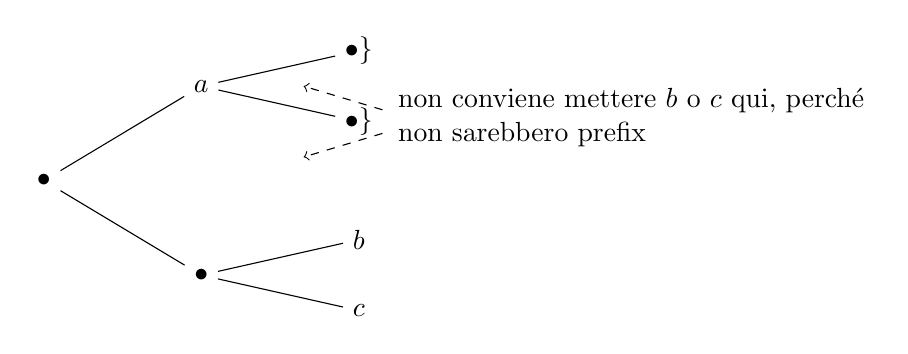
\begin{tikzpicture}[grow=right]
        \tikzstyle{level 2}=[sibling distance=.9cm]
        \node {$\bullet$}
        child {
            node {$\bullet$}
            child {
                node {$c$}
                edge from parent
            }
            child {
                node {$b$}
                edge from parent
            }    
            edge from parent
        }
        child {
            node {$a$}
            child {
                node {$\bullet\}$}
                edge from parent
            }
            child {
                node {$\bullet\}$}
                edge from parent
            }
            edge from parent
        };
    \node[text width=6cm,align=left] at (7.5,.8) {non conviene mettere $b$ o $c$ qui, perché non sarebbero prefix};
    \draw[->] (4.3,.9) node {} -- (3.3,1.2) [dashed] node {};
    \draw[->] (4.3,.6) node {} -- (3.3,.3) [dashed] node {};
    \end{tikzpicture}
\end{center}

\begin{theorem}[Teorema Diretto]
    $$
        \sum_{i=1}^k D^{-l_i} \leq 1
        \quad \Rightarrow \quad
        \exists \varphi \text{ prefisso con lunghezze } l_1,\dots,l_k
    $$
\end{theorem}
Prefisso è più forte di UD.\medskip 

I due risultati (teoremi) affermano che, anche se ci limitiamo all'utilizzo di codici prefisso, non perdiamo alcuna potenza nella compressione. È sufficiente l'utilizzo dei codici prefisso, comprimono a sufficienza.

\paragraph{Dimostrazione Teorema Inverso, caso prefisso + Teorema Diretto} Sia $\varphi$ un codice prefisso e $l_1\leq l_2\leq\dots\leq l_k=l$. Consideriamo l'albero $D$-ario (ogni nodo ha $D$ figli) che rappresenta $\varphi$, di altezza $l$.
\begin{center}
    \begin{tikzpicture}[grow=right]
        \tikzstyle{level 2}=[sibling distance=.5cm]
        \node {$\bullet$}
        child {
            node {$\bullet$}
            child {
                [dotted] node[right] {$\dots\bullet$}
                edge from parent
            }
            child {
                [dotted] node[right] {$\dots\bullet$}
                edge from parent
            }
            child {
                [dotted] node[right] {$\dots\bullet$}
                edge from parent
            }    
            edge from parent
        }
        child {
            node {$\bullet$}
            child {
                [dotted] node[right] {$\dots\bullet$}
                edge from parent
            }
            child {
                [dotted] node[right] {$\dots\bullet$}
                edge from parent
            }
            child {
                [dotted] node[right] {$\dots\bullet$}
                edge from parent
            }
            edge from parent
        }
        child {
            node {$\bullet$}
            child {
                [dotted] node[right] {$\dots\bullet$}
                edge from parent
            }
            child {
                [dotted] node[right] {$\dots\bullet$}
                edge from parent
            }
            child {
                [dotted] node[right] {$\dots\bullet$}
                edge from parent
            }
            edge from parent
        };
    \draw[<->] (4,-2.5) node {} -- (0,-2.5) node {};
    \node[below] at (2,-2.5) {$l$};
    \end{tikzpicture}
\end{center}

La codifica più lunga $a_k$ è in una delle foglie. Supponiamo che la codifica $a_i$ sia in uno dei nodi interni. Nessuno dei nodi interni (e in particolare nessuna delle foglie) del sottoalbero con $a_i$ come radice può essere utilizzato per un'altra codifica.
\begin{center}
    \begin{tikzpicture}[grow=right]
        \tikzstyle{level 1}=[level distance=2cm,sibling distance=2.4cm]
        \tikzstyle{level 2}=[level distance=2cm,sibling distance=.8cm]
        \node {$\bullet$}
        child {
            node {$\bullet$}
            child {
                [dotted] node[right] {$\qquad\dots\qquad\bullet$}
                edge from parent
            }
            child {
                [dotted] node[right] {$\qquad\dots\qquad\bullet$}
                edge from parent
            }
            child {
                [dotted] node[right] {$\qquad\dots\qquad\bullet$}
                edge from parent
            }    
            edge from parent
        }
        child {
            node {$\bullet$}
            child {
                [dotted] node[right] {$\qquad\dots\qquad\bullet$}
                edge from parent
            }
            child {
                [dotted] node[right] {$\qquad\dots\qquad a_k$}
                edge from parent
            }
            child {
                [dotted] node[right] {$\qquad\dots\qquad\bullet$}
                edge from parent
            }
            edge from parent
        }
        child {
            node {$\bullet$}
            child {
                [dotted] node[right] {$a_i$}
                edge from parent
            }
            child {
                [dotted] node[right] {$\qquad\dots\qquad\bullet$}
                edge from parent
            }
            child {
                [dotted] node[right] {$\qquad\dots\qquad\bullet$}
                edge from parent
            }
            edge from parent
        };
        \node[isosceles triangle,
            isosceles triangle apex angle=30,
            draw,
            rotate=180,
            fill=Gray!30,
            minimum size=1cm] (T)at (6.1,1.65){};
        \node at (5.8,1.65) {\tiny VIETATO};
    \end{tikzpicture}
\end{center}
In un tale albero, il numero di foglie è pari a $D^l$. 
\begin{center}
    \begin{tikzpicture}[grow=right]
        \tikzstyle{level 2}=[sibling distance=.5cm]
        \node {$\bullet$}
        child {
            node {$\bullet$}
            child {
                [dotted] node[right] {$\dots\bullet$}
                edge from parent
            }
            child {
                [dotted] node[right] {$\dots\bullet$}
                edge from parent
            }
            child {
                [dotted] node[right] {$\dots\bullet$}
                edge from parent
            }    
            edge from parent
        }
        child {
            node {$\bullet$}
            child {
                [dotted] node[right] {$\dots\bullet$}
                edge from parent
            }
            child {
                [dotted] node[right] {$\dots\bullet$}
                edge from parent
            }
            child {
                [dotted] node[right] {$\dots\bullet$}
                edge from parent
            }
            edge from parent
        }
        child {
            node {$\bullet$}
            child {
                [dotted] node[right] {$\dots\bullet$}
                edge from parent
            }
            child {
                [dotted] node[right] {$\dots\bullet$}
                edge from parent
            }
            child {
                [dotted] node[right] {$\dots\bullet$}
                edge from parent
            }
            edge from parent
        };
    \draw[<->] (4.5,-2.1) node {} -- (4.5,2.1) node {};
    \node[right] at (4.5,0) {$D^l$};
    \end{tikzpicture}
\end{center}
Il numero di foglie di un sottoalbero che parte da un nodo interno $a_i$ è $D^{l-l_i}$.
\begin{center}
\begin{tikzpicture}
    \node[isosceles triangle,
        isosceles triangle apex angle=40,
        draw,
        rotate=180,
        fill=Gray!30,
        minimum size=2.5cm] (T)at (0,0){};
    \draw[<->] (-2.55,-1.5) node {} -- (.85,-1.5) node {};
    \node[below] at (-0.85,-1.5) {$l-l_i$};
    \node at (-2.55,0) {$\bullet$};
    \node[left] at (-2.55,0) {$a_i$};
    \node[right] at (.85,1) {$\bullet$};
    \node[right] at (.85,0.1) {$\vdots$};
    \node[right] at (.85,-1) {$\bullet$};
    \draw[<->] (1.6,1.25) node {} -- (1.6,-1.25) node {};
    \node[right] at (1.6,0) {$D^{l-l_i}$};
\end{tikzpicture}
\end{center}
Quindi, riassumendo:
\begin{center}
    \begin{tikzpicture}[grow=right]
        \tikzstyle{level 1}=[level distance=2cm,sibling distance=2.4cm]
        \tikzstyle{level 2}=[level distance=2cm,sibling distance=.8cm]
        \node {$\bullet$}
        child {
            node {$\bullet$}
            child {
                [dotted] node[right] {$\qquad\dots\qquad\bullet$}
                edge from parent
            }
            child {
                [dotted] node[right] {$\qquad\dots\qquad\bullet$}
                edge from parent
            }
            child {
                [dotted] node[right] {$\qquad\dots\qquad\bullet$}
                edge from parent
            }    
            edge from parent
        }
        child {
            node {$\bullet$}
            child {
                [dotted] node[right] {$\qquad\dots\qquad\bullet$}
                edge from parent
            }
            child {
                [dotted] node[right] {$\qquad\dots\qquad a_k$}
                edge from parent
            }
            child {
                [dotted] node[right] {$\qquad\dots\qquad\bullet$}
                edge from parent
            }
            edge from parent
        }
        child {
            node {$\bullet$}
            child {
                [dotted] node[right] {$a_i$}
                edge from parent
            }
            child {
                [dotted] node[right] {$\qquad\dots\qquad\bullet$}
                edge from parent
            }
            child {
                [dotted] node[right] {$\qquad\dots\qquad\bullet$}
                edge from parent
            }
            edge from parent
        };
        \node[isosceles triangle,
            isosceles triangle apex angle=30,
            draw,
            rotate=180,
            fill=Gray!30,
            minimum size=1cm] (T)at (6.1,1.65){};
        \draw[<->] (-.1,-4) node {} -- (6.4,-4) node {};
        \node[below] at (3.15,-4) {$l$};
        \draw[<->] (6.8,1.15) node {} -- (6.8,2.15) node {};
        \node[right] at (6.8,1.65) {$D^{l-l_i}$};
        \draw[<->] (8.2,-3.3) node {} -- (8.2,3.3) node {};
        \node[right] at (8.2,0) {$D^l$};
    \end{tikzpicture}
\end{center}
Scriviamo che la differenza tra il numero totale di foglie $D^l$ e il numero di foglie dei sottoalberi (ovvero il numero di foglie vietate a causa dei sottoalberi creati da ogni $a_i$) è maggiore o uguale a 1:
\begin{align*}
    D^l - \sum_{i=1}^{k-1} D^{l-l_i} & \geq 1\\
    D^l\left(1-\sum_{i=1}^{k-1} D^{-l_i}\right) & \geq 1\\
    1 - \sum_{i=1}^{k-1} D^{-l_i} & \geq D^{-l_k}\\
    1 & \geq \sum_{i=1}^k D^{-l_i} %\qquad \square
\end{align*}
\hfill $\square$\medskip

Per il \textbf{Teorema Diretto}, si può leggere la dimostrazione ``al contrario''. In altre parole, vengono date le istruzioni per costruire l'albero, ovvero si disegna l'albero completo e si inizia ad etichettare. Più precisamente, si prende $a_1$, lo si mette a lunghezza $l_1$, e fino alle foglie si segna il resto dell'albero (il sottoalbero con radice $a_1$) come vietato. Si continua così per tutti gli $a_i$. \hfill $\square$

\paragraph{Dimostrazione Teorema Inverso, caso $\bm{\varphi}$ UD} Siano $l_1\leq\dots\leq l_k=l$ le lunghezze delle codifiche di $a_1,\dots,a_k$. Consideriamo $\mathcal{N}(n,h)$ numero di stringhe su $\mathcal{A}^n$ (ovvero di lunghezza $n$) che hanno una codifica $\varphi$ UD di lunghezza $h$. Sia $|\mathcal{B}^h|=D^h$ (numero di stringhe di lunghezza $h$ su $\mathcal{B}$). Poiché $\varphi$ è UD, $\mathcal{N}(n,h)\leq D^h$.
$$
    \sum_{i=1}^k D^{-l_i} = D^{-l_1} + D^{-l_2} + \dots + D^{-l_k} 
$$

Studiamo la crescita di tale oggetto alla potenza di $n$, quando $n$ va ad infinito. Questo perché, se la somma è $>1$, allora la potenza va ad infinito; se la somma è $<1$, allora la potenza va a 0 (è limitata); se la somma è $=1$, allora la potenza va a 1.
$$
    \forall n \qquad \left(D^{-l_1} + D^{-l_2} + \dots + D^{-l_k}\right)^n \qquad (\text{chiamiamola }\alpha^n)
$$

Se si svolge l'elevamento a potenza di tale polinomio, si otterrà una serie di addendi del seguente tipo:
$$
    D^{-l_1\cdot n} +
    \dots +
    D^{(-l_1)+(-l_2)+(-l_1)+\dots} +
    \dots +
    D^{-l_k\cdot n}
$$
dove $-l_1\cdot n$ è la lunghezza della codifica della stringa $a_1a_1\dots a_1$, con $n$ ripetizioni di $a_1$, ovvero $|\varphi(a_1\dots a_1)|=l_1\cdot n$. Allo stesso modo, $-l_k\cdot n$ è la lunghezza della codifica della stringa $a_ka_k\dots a_k$, con $n$ ripetizioni di $a_k$. Un generico esponente all'interno, ad esempio $-(l_1+l_2+l_1+\dots)$ è una somma di lunghezze di codifiche, e ammonta alla lunghezza di una generica stringa. Ad esempio, $-(10)$, se chiamo $10=h$.

Si ha che $D^{-h}$ si verifica nella somma esattamente $\mathcal{N}(n,h)$ volte (alcune delle quali saranno 0). Quindi, la somma $D^{-l_1\cdot n}+\dots+D^{-l_k\cdot n}$ si può riscrivere come 
\begin{align*}
    \mathcal{N}(n,0)D^{-0} + \mathcal{N}(n,1)D^{-1} + \dots + \underbrace{\mathcal{N}(n,n\cdot l)}_{\geq 1}D^{-n\cdot l} & \quad\leq\quad
    D^0D^{-0} + D^1D^{-1} + \dots + D^{n\cdot l}D^{-n\cdot l}\\
    1+1+\dots+1 & \quad\leq\quad n\cdot l + 1\\
    \forall n \qquad \alpha^n &\quad\leq\quad \underbrace{l}_{costante}\cdot~ n
\end{align*}
Da cui si ricava
$$
    \alpha \leq 1
$$
Quindi
$$
    \sum_{i=1}^k D^{-l_i} \leq 1
$$
\hfill $\square$



\section{Compressione Massima}
La sorgente che genera il messaggio del codice è stazionaria e senza memoria (Fig.~\vref{fig:shannon-paper}).
\begin{figure}[htb]
    \centering
    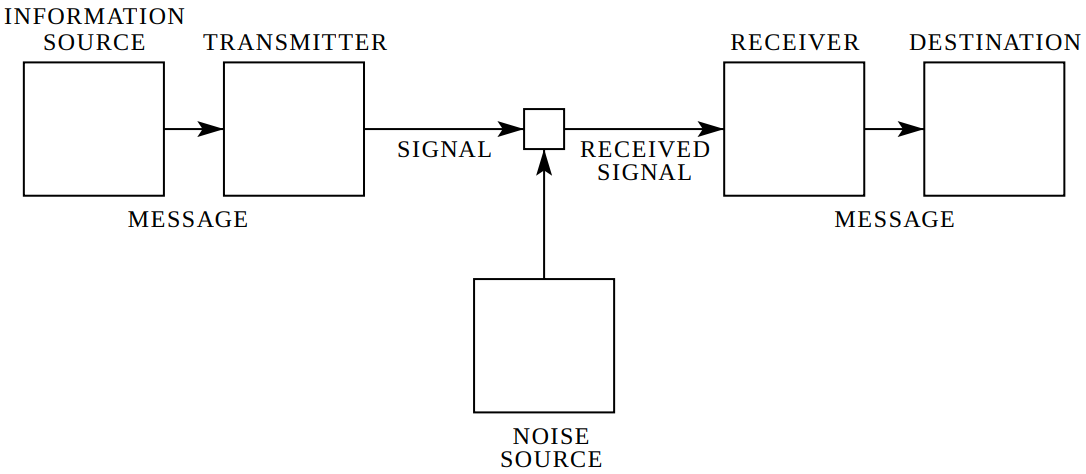
\includegraphics[width=.7\textwidth]{figures/shannon-paper.png}
    \caption{Diagramma schematico di un sistema di comunicazione, da C.~E.~Shannon, \textit{A Mathematical Theory of Communication}, Bell System Technical Journal, 1948.}
    \label{fig:shannon-paper}
\end{figure}
Poiché il messaggio codificato deve passare attraverso un canale, il quale ha una sua capacità e una sua velocità, lo si vuole comprimere il più possibile.

Ricordiamo che 
$$
    P=\{p_1,\dots,p_k\} \qquad \mathcal{A}=\{a_1,\dots,a_k\} \qquad l_i=|\varphi(a_i)| \qquad EL(\varphi) = \sum_{i=1}^k p_il_i
$$

\begin{theorem}[$\bm{1^\circ}$ Shannon]
    $$
        \varphi \text{ è UD} \quad \Rightarrow \quad EL(\varphi) \geq \mathcal{H}_D(P)
    $$

    con 
    $$
        \mathcal{H}_D(P) = \sum_{i=1}^k p_i\cdot\log_D\frac{1}{p_i}
    $$
\end{theorem}

\paragraph{Dimostrazione} 
\begin{align*}
    EL(\varphi)-\mathcal{H}_D(P) &= \sum_{i=1}^k p_i\underbrace{l_i}_{\log_DD^{l_i}} + \sum_{i=1}^k p_i\cdot\log_Dp_i\\
    &= \sum_{i=1}^k p_i\cdot\log_D(D^{l_i}\cdot p_i)\\
\end{align*}
Prima di proseguire, ricordiamo la seguente proprietà dei logaritmi su $\mathbb{N}$:
$$
    \log_ex\leq x-1; \qquad -\log_ex\geq -(x-1) 
$$
e anche la proprietà dei logaritmi:
$$
    \log_bx = \frac{\log_cx}{\log_cb}
$$
Continuiamo la dimostrazione:
\begin{align*}
    EL(\varphi)-\mathcal{H}_D(P) &= \sum_{i=1}^k p_i\cdot\log_D(D^{l_i}\cdot p_i)\\
    &= \frac{1}{log_eD} \sum_{i=1}^k p_i\cdot\log_e(D^{l_i}\cdot p_i)\\
    &= -\frac{1}{\log_eD} \sum_{i=1}^k p_i\cdot\log_e\left(\frac{1}{D^{l_i}\cdot p_i}\right)\\
    &\geq -\frac{1}{\log_eD} \sum_{i=1}^k p_i\cdot\left(\frac{1}{D^{l_i}\cdot p_i}-1\right)\\
    &= -\frac{1}{\log_eD} \underbrace{\left(\sum_{i=1}^k\frac{1}{D^{l_i}}-\underbrace{1}_{\sum p_i}\right)}_{\leq 0}\\
    &\geq 0
\end{align*}
\hfill $\square$ 


% LEZIONE 5
\section{Shannon Code}
Dal Teorema $1^\circ$ Shannon abbiamo:
$$
EL(\varphi) = \sum_{i=1}^k p_il_i ~ \geq ~ \mathcal{H}_D(P) = \sum_{i=1}^k p_i\log_D\frac{1}{p_i}
$$
La differenza sta in $l_i$ e $\log_D\frac{1}{p_i}$, quindi vogliamo provare ad eguagliarli:
$$
    l_i = \log_D\frac{1}{p_i}
$$
Ma $\log_D\frac{1}{p_i}$ non è necessariamente intero. Decidiamo quindi di considerare il suo primo intero più grande:
$$
l_i = \left\lceil\log_D\frac{1}{p_i}\right\rceil = \left\lceil-\log_Dpi\right\rceil
$$
È sempre possibile definire un codice UD con tali lunghezze? Possiamo utilizzare Kraft-McMillan. Vogliamo controllare se
$$
    \sum_{i=1}^k D^{-\lceil-\log_Dpi\rceil}
    \stackrel{?}{\leq}
    1
$$
Sappiamo che 
$$
    \lceil-\log_Dpi\rceil = -log_Dp_i+\beta_i \qquad\qquad 0\leq\beta_i<1
$$
Quindi possiamo scrivere
\begin{align*}
    \sum_{i=1}^k D^{-(-log_Dp_i+\beta_i)} &= \sum_{i=1}^k D^{log_Dp_i}\cdot D^{\beta_i}\\
    &= \sum_{i=1}^k p_i\cdot D^{-\beta_i}\\
    &= \sum_{i=1}^k p_i\cdot \frac{1}{D^{\beta_i}}
\end{align*}
Ricordiamo che $0\leq\beta_i<1$ e $D>1$, di conseguenza $\frac{1}{D^{\beta_i}}\leq 1$. Quindi
\begin{align*}
    \sum_{i=1}^k p_i\cdot \frac{1}{D^{\beta_i}} &\leq 1\\
    \sum_{i=1}^k D^{-\lceil-\log_Dpi\rceil} &\leq 1
\end{align*}
Esiste quindi un prefix code con lunghezze $l_i=\lceil-\log_Dpi\rceil$ definibile utilizzando una strategia greedy sull'albero $D$-ario.
\begin{center}
    \begin{tikzpicture}[grow=right]
        \tikzstyle{level 1}=[level distance=2cm,sibling distance=2cm]
        \tikzstyle{level 2}=[level distance=2cm,sibling distance=1.2cm]
        \node {$\bullet$}
        child {
            [dotted] node { }
            edge from parent
        }
        child {
            node {$\bullet$}
            edge from parent
        }
        child {
            node {$\bullet$}
            child {
                [dotted] node[right] { }
                edge from parent
            }
            child {
                [dotted] node[right] { }
                edge from parent
            }
            child {
                [dotted] node[right] {$\varphi(a_1)$}
                edge from parent
            }
            edge from parent
        };

        \draw [decorate,
            decoration = {brace,amplitude=10pt}] (-0.2,0.3) -- (3.8,3.5);
        \node[rotate=40] at (1.3,2.4) {$\lceil-\log_Dpi\rceil$};
    \end{tikzpicture}
\end{center}

\textcolor{Red}{TODO: finire lezione 5}


% LEZIONE 6
\begin{definition}[Efficienza (Efficiency of code)]
    $$
        Eff(\varphi) = \frac{\mathcal{H}_D(P)}{EL(\varphi)}
    $$
\end{definition}
\emph{Eff} è sempre $\leq 1$, e ci dice quanto siamo vicini all'entropia, che non è sempre raggiungibile.\medskip

Ci chiediamo perché Huffmann (merge delle foglie) è ottimale, mentre Shannon-Fano (splitting dalla radice) non lo è?


\section{Lempel-Ziv}
\textcolor{Red}{TODO: scrivere la storia}


\subsection{LZ77}

